\documentclass[oribibl]{llncs}
\usepackage[utf8]{inputenc}
\usepackage{llncsdoc}
\usepackage{url}
\usepackage{amsmath}
\usepackage{amssymb}
\usepackage{graphicx}
\usepackage{wrapfig}
\usepackage[cache=false,outputdir=.texpadtmp]{minted}

%
\author{Lennard Wolf \\
        lennard.wolf@student.hpi.de}
\institute{ Hasso Plattner Institute \\
            Prof.-Dr.-Helmert-Straße 2-3 \\
            14482 Potsdam \\
            Germany}
\title{Describing Dynamic Organizational Structures \\
 with the Common Lisp Object System}
\date{\today}
%
\begin{document}
\markboth{Describing Dynamic Organizational Structures \\
 with the Common Lisp Object System}{Describing Dynamic Organizational Structures \\
 with the Common Lisp Object System}
\thispagestyle{empty}
\vfill

%
\maketitle
%
\begin{abstract}
CLOS is an object-oriented system for Common Lisp. In this work, we present its history, basic syntax, as well as its three main concepts of \emph{multiple inheritance}, \emph{method combination}, and \emph{generic functions}. This is done by showing their application to the domain of descriptions of organizational structures. The university is used as example use case and the implementation of a maintainable, extendable, and accessible framework to describe its structure is presented.

\end{abstract}
%


\section{Introduction}

Organizational structures often require maintainable and easily extendable descriptions of shareholders and their roles. The \emph{Common Lisp Object System} (CLOS) with its concepts of \emph{multiple inheritance}, \emph{generic functions}, and \emph{method combination} is a tool that facilitates the creation and perpetuation of such a register of members. This work presents an overview of CLOS' history as well as its basic syntax and core concepts by employing it for the creation of a dynamic member register for a university. 
\newline

This work is structured as follows. Section \ref{sec:problem} introduces the problem of dynamic shareholder lists for organizational structures. Section \ref{sec:background} introduces CLOS, its history, and core concepts. In Section \ref{sec:approach}, CLOS is applied to the given problem, first in theory, then in practice. Section \ref{sec:evaluation} gives a short evaluation of the solution based on the given criteria, in Section \ref{sec:related}, a different solution using Java is discussed, and Section \ref{sec:conclusion} concludes this work.


\section{Problem}
\label{sec:problem}

To achieve their goals, organizational structures require planning as well as control over processes and the network of shareholders \cite[42f.]{Schmidt2000}. To gain the necessary overview, it is often useful to have a list of all members and their roles. In the United Kingdom\footnote{Companies Act 2006 \url{http://legislation.data.gov.uk/ukpga/2006/46/part/8/chapter/2/data.htm?wrap=true}, accessed: 2016-07-18} as well as other countries such a \emph{register of members} is furthermore required by the legislation.

Since organizations are often dynamic, such a list should also be easily \emph{maintainable}, meaning that participants can be both added or removed as well as change their role. It should also be \emph{extendable} meaning that new roles can easily added and combined with already existing ones. Furthermore, computer programs used within the organization might have to interact with the list, so \emph{accessibility} is another key requirement. These \emph{evolution qualities} \cite{young2001effective} would thus be the key requirements for  any list describing the participants within an organizational structure.


\section{Background}
\label{sec:background}
A solution to the problem introduced in Section \ref{sec:problem} which would meet all the given requirements would be the employment of the Common Lisp Object System, an extension to Common Lisp\footnote{\url{https://common-lisp.net}, accessed: 2016-07-12} providing Object Orientation \cite{demichiel1987common}. However, to understand its utilization in such a problem domain, as well as the reasoning behind that, some background information will be needed first.

In this Section we will hence start out by introducing the general ideas behind object-orientated programming languages, as well as the language Lisp, which is followed by a description of the three main concepts that make CLOS unique. An overview of the history of CLOS will be provided thereafter, so as to better understand its origins and historical context.

\subsection{Object-Oriented Languages}
\label{sec:oo}

At its core, Object Orientation is a concept in computer science, after which a program works in such a way that it is made up of individual objects that can interact with one another. This \emph{paradigm} can be implemented into a language in different ways. But next to such variations such as prototype-based programming, the quintessential Object Orientation style is class-based, according to \cite{wegner1987dimensions}, which we refer to in the following  definition.

A definition of \emph{object-oriented} programming languages requires a preceding explanation of the terms \emph{object}, \emph{class}, and \emph{inheritance}. \emph{Objects} have a set of \emph{attributes} that define its \emph{state}, as well as a number of \emph{messages} that it can receive to evoke certain behavior, defined by \emph{methods}. By sending such messages, objects can interact with one another. \emph{Classes} are templates for objects, so that objects of the same class can have uniform interfaces and behavior. An object is hence an \emph{instance} of a class. \emph{Inheritance} opens up the possibility to create class hierarchies, so that classes can be specializations of others and \emph{inherit} certain behavior while adding something unique. The inheriting class is called the \emph{subclass}, the other the \emph{superclass}. \cite{wegner1987dimensions}

An \emph{object-oriented} programming language is one that has these three concepts "integrated". They give programmers the ability to model human language based conceptualizations of the real world, since these are also just separations of phenomena into groups with common traits.

\subsection{Lisp}
\label{sec:lisp}

Stemming from the term \textbf{Lis}t \textbf{P}rocessor, Lisp is a programming language in which \emph{everything is a list}. This means that there is \emph{no discernment between data and code}. Hence an expression such as \mintinline{lisp}{(plus 3 4)} is without context nothing more than a "meaningless" listing of the "meaningless" expressions \mintinline{lisp}{plus}, \mintinline{lisp}{3}, and \mintinline{lisp}{4}. An expression like that only gets its meaning from an \emph{evaluation} by the interpreter which considers it in a certain context. In such a context the expression \mintinline{lisp}{plus} could be a function to add the arguments it is given, but that is entirely arbitrary. 

Common Lisp is a standardized version of Lisp which provides certain data types and operations. But this type system can be extended through the use of \emph{macros}, which let developers give meaning to expressions. This can be demonstrated by a trivial example. By defining a macro \mintinline{lisp}{(defmacro eight () (+ 3 5))}, a programmer would be able to simply write \mintinline{lisp}{eight} instead of the actual number whenever it is needed in the code. In the \emph{macro expansion phase} during compilation, the compiler then replaces all occurrences of \mintinline{lisp}{eight} with \mintinline{lisp}{(+ 3 5)}, which, during evaluation, will turn into the desired number. This feature of the Lisp language enables programmers to interfere with evaluation orders, and also greatly facilitates the creation of \emph{Domain Specific Languages} \cite{fowler2011domain-specific}. Furthermore, they form the basis of CLOS which in its entirety consists of 8 macros and 33 functions.


\subsection{History of CLOS}
\label{sec:history}

In the late 1960s, the new concept of Object Orientation started to become a topic of interest for researchers in computer science. In 1986, four major attempts, namely New Flavors\footnote{Information on its predecessor Flavors can be found in \cite{Moon:1986:OPF:28697.28698}.}, CommonLoops\footnote{Information on CommonLoops can be found in \cite{Bobrow:1986:CML:28697.28700}.}, Object Lisp (LMI), and Common Objects, were made to bring that concept to the popular and easily extendable programming language Lisp \cite{steele1993evolution}. To create a standardized object system, researchers from Symbolics, Inc. and Xerox PARC met to combine their respective object systems, New Flavors and CommonLoops \cite{demichiel1987common}. The Common Lisp Object System was the result, which had been two years in the making \cite{steele1993evolution}. Important concepts, next to those described in the following \emph{Main Concepts} passage, were \emph{metaclasses}, of which regular classes are just instances, and \emph{metaobjects}, which lay the foundation for the concept of objects\cite{kiczales1991art}. The \emph{metaobject protocol} in CLOS allows the system to be written in itself \cite{steele1993evolution}. Furthermore, CLOS is portable to different LISP dialects. Examples are \emph{EIEIO}\footnote{\url{https://www.gnu.org/software/emacs/manual/html_mono/eieio.html}, accessed: 2016-07-13} for Emacs Lisp and \emph{SOS}\footnote{\url{https://www.gnu.org/software/mit-scheme/documentation/mit-scheme-sos/}, accessed: 2016-07-13} for Scheme.

\subsection{Main Concepts}
\label{sec:concepts}

CLOS comprises concepts that are rather uncommon in modern object-oriented languages. This is, in the cases of \emph{generic functions} and \emph{method combination}, due to their specificity to the Lisp environment and, in the case of \emph{multiple inheritance}, because it can cause many problems if employed in contexts that are inappropriate, which they more often than not are \cite{cargill1993case}. We will thus start out if a short introduction of the new macros supplied by CLOS, which we will then need to explain the aforementioned concepts.


\subsubsection{Syntax Basics}
The core of object-oriented programming lies with the creation of classes, corresponding methods, and the instantiation of objects. Listing \ref{lst:clossyntax} shows these basic operations in CLOS. Other macros exist\footnote{The entire implementation of CLOS can be found at \url{http://norvig.com/paip/clos.lisp}, accessed: 2016-07-13} but are not relevant in this context.

\begin{listing}[]%ht]
\begin{minted}{lisp}
;;; Generic form of class and method definition, as well as instantiation
(defclass NAME (SUPERCLASS1 ... SUPERCLASSn) (ATTRIBUTES))

(defmethod NAME (RECIPIENT1 ... RECIPIENTn) (CODE))

(make-instance 'CLASS :ATTR1 VAL1 ... :ATTRn VALn)
\end{minted}
\caption{The central macros provided by CLOS}
\label{lst:clossyntax}
\end{listing}


\subsubsection{Multiple Inheritance}
\label{sec:mulinh}
was first introduced by the predecessor of New Flavors, \emph{Flavors}. It allows classes to have multiple superclasses, thereby inheriting methods and attributes of each (see Figure \ref{fig:multipleinheritance}). The AthleticTeacher class defined by \mintinline{lisp}{(defclass athletic-teacher (teacher athlete) () )} would, if some inheritances from Teacher and Athlete are conflicting, prioritize the Teacher behavior, because it is listed first.  

\begin{figure}[]
    \centering
    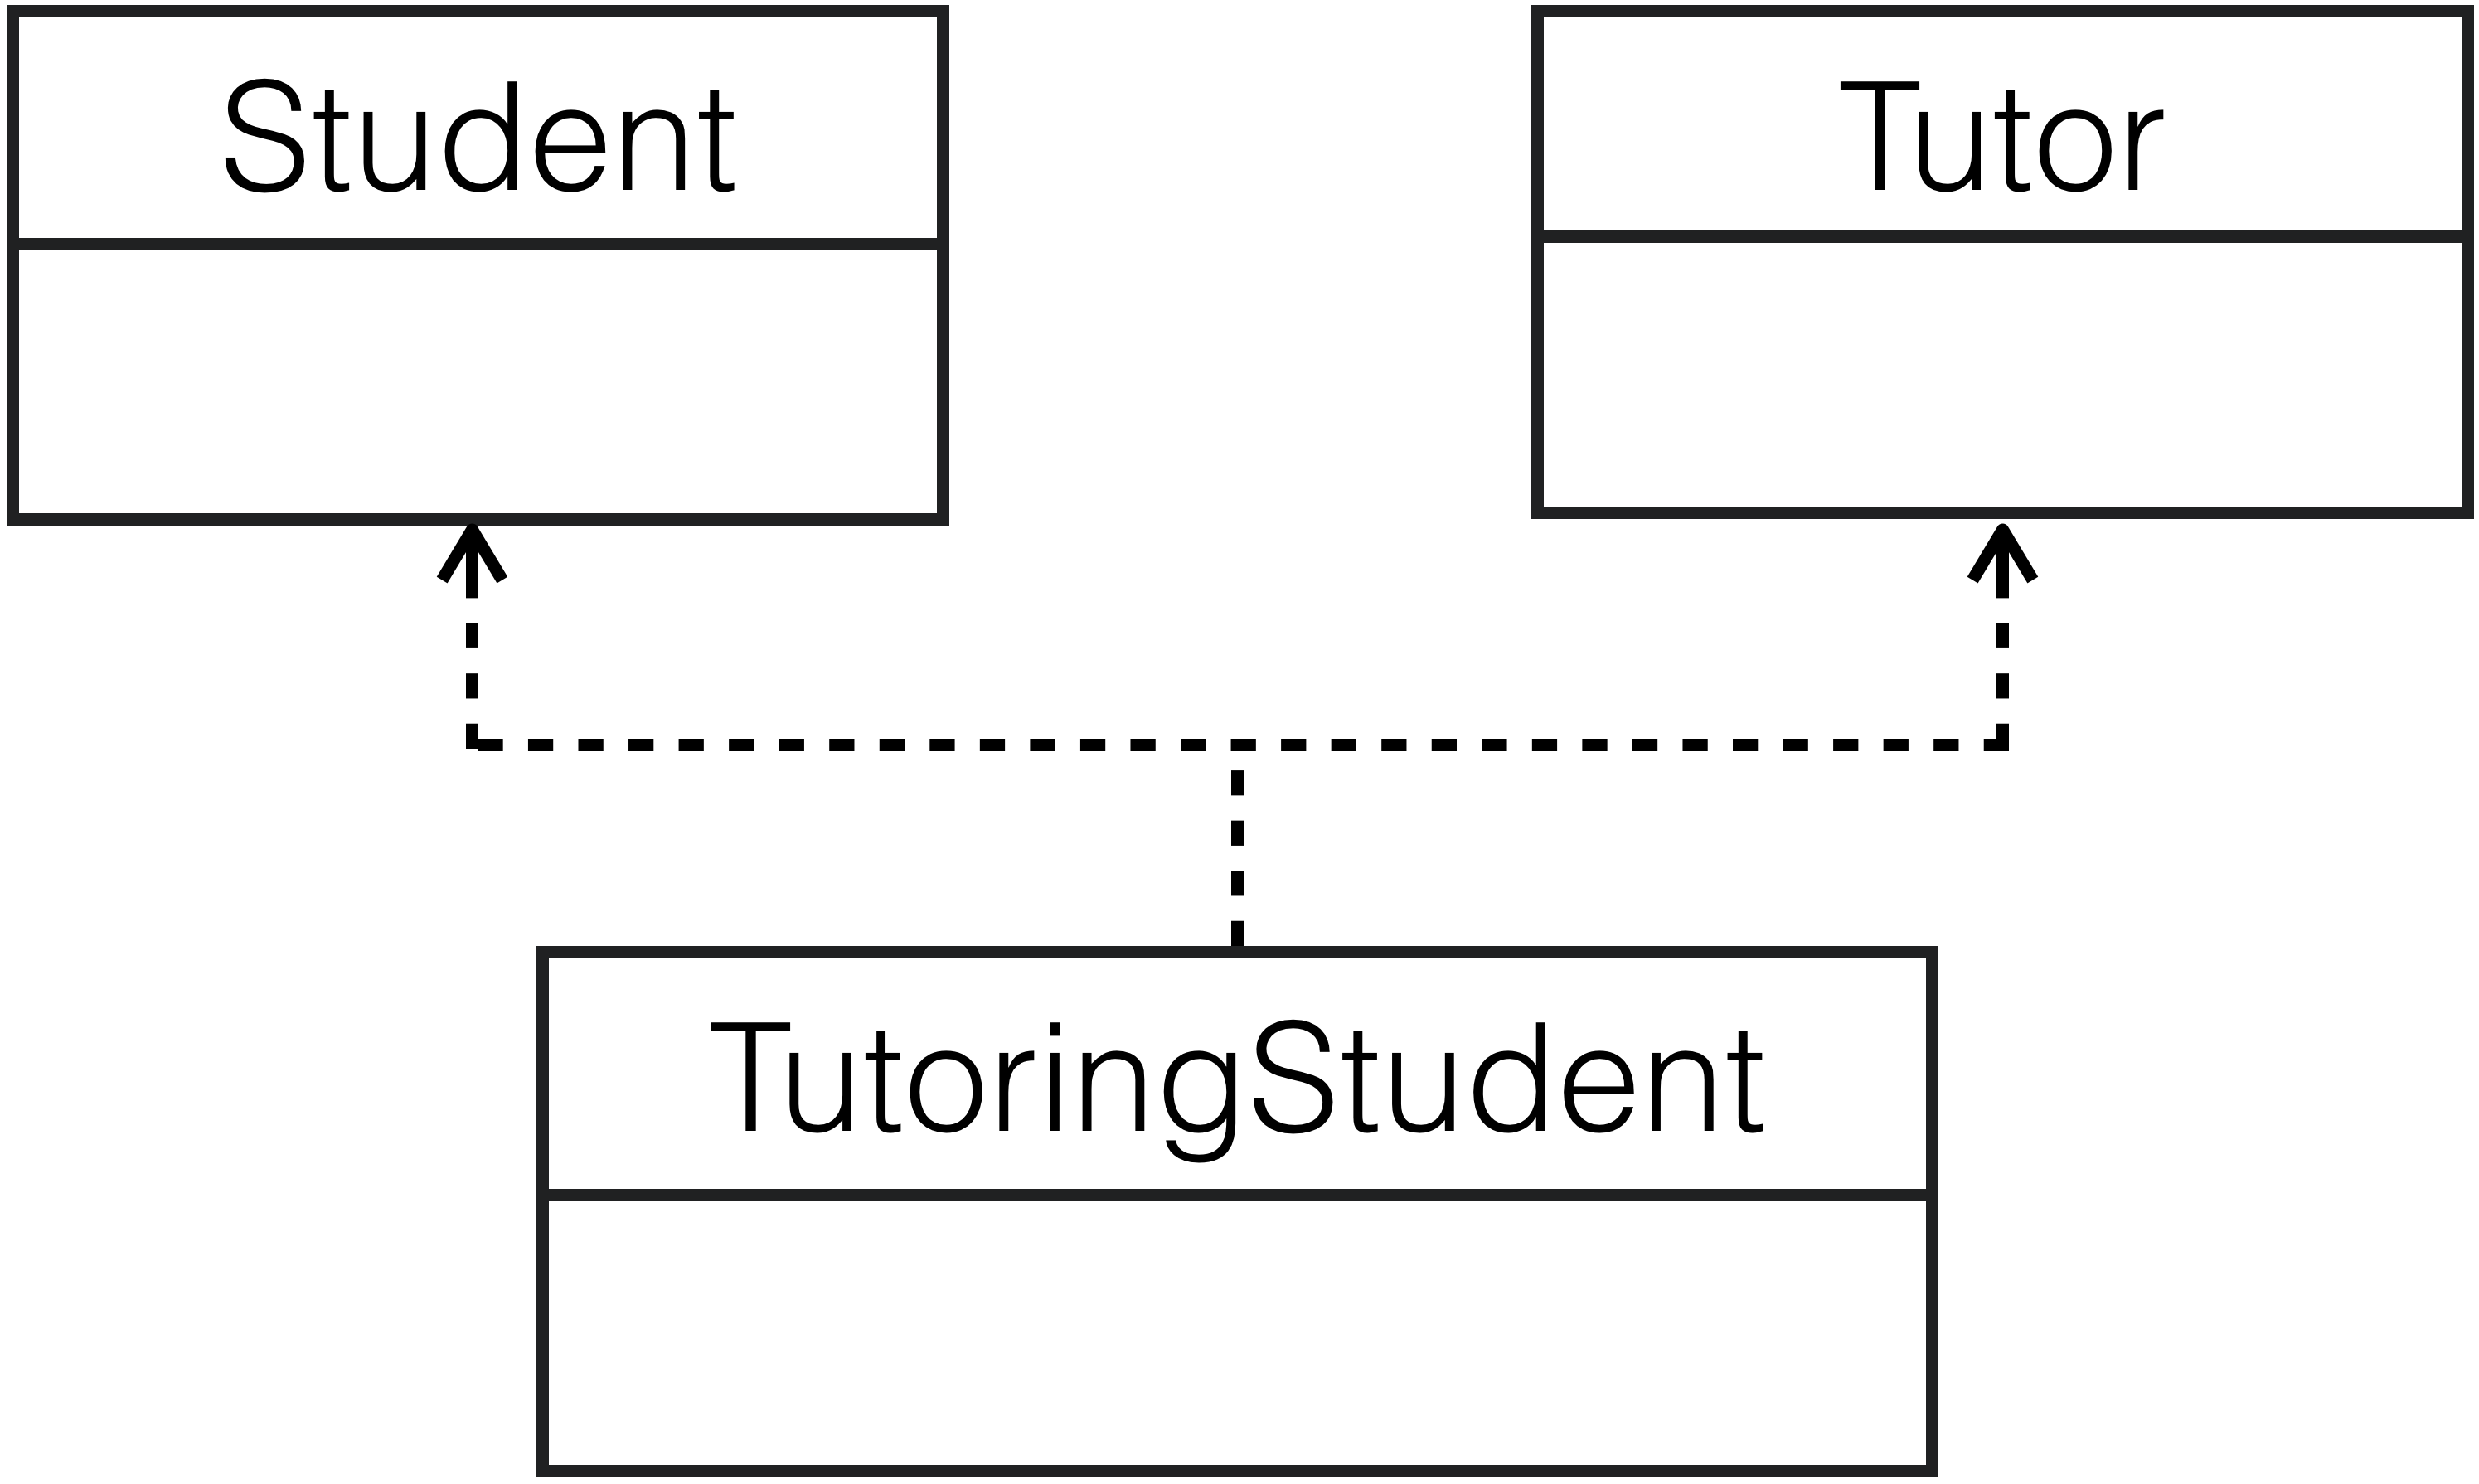
\includegraphics[width=0.35\textwidth]{images/multipleinheritance2.png}
    \caption{A UML class diagram with multiple inheritance}
    \label{fig:multipleinheritance}
\end{figure}

\subsubsection{Method Combination}
\label{sec:metcom}
is an important addition to multiple inheritance, because it lets developers blend behavior together. The keywords \mintinline{lisp}{:before}, \mintinline{lisp}{:after}, and \mintinline{lisp}{:around} allow the specification of certain behavior to be added to a called method. \mintinline{lisp}{(defmethod method :after}\mintinline{lisp}{ ((teach teacher))}
    \mintinline{lisp}{()} would run additional behavior after the primary behavior defined for \mintinline{lisp}{method} for all Teacher. 


\subsubsection{Generic Functions}
\label{sec:genfun}
In Flavors, messages were sent to objects by calling the \mintinline{lisp}{send} function \mintinline{lisp}{(send object :message)}. New Flavors however introduced the \mintinline{lisp}{(message object)} notation, which required \mintinline{lisp}{message} to be \emph{generic}, meaning that it needed to be a globally defined interface (see Figure \ref{fig:genericfunction}). By calling the generic function, different behavior will ensue, depending on the type of the receiver provided as argument. If methods are defined that have no corresponding generic function, CLOS will add it automatically at compile time.


\begin{figure}[]
    \centering
    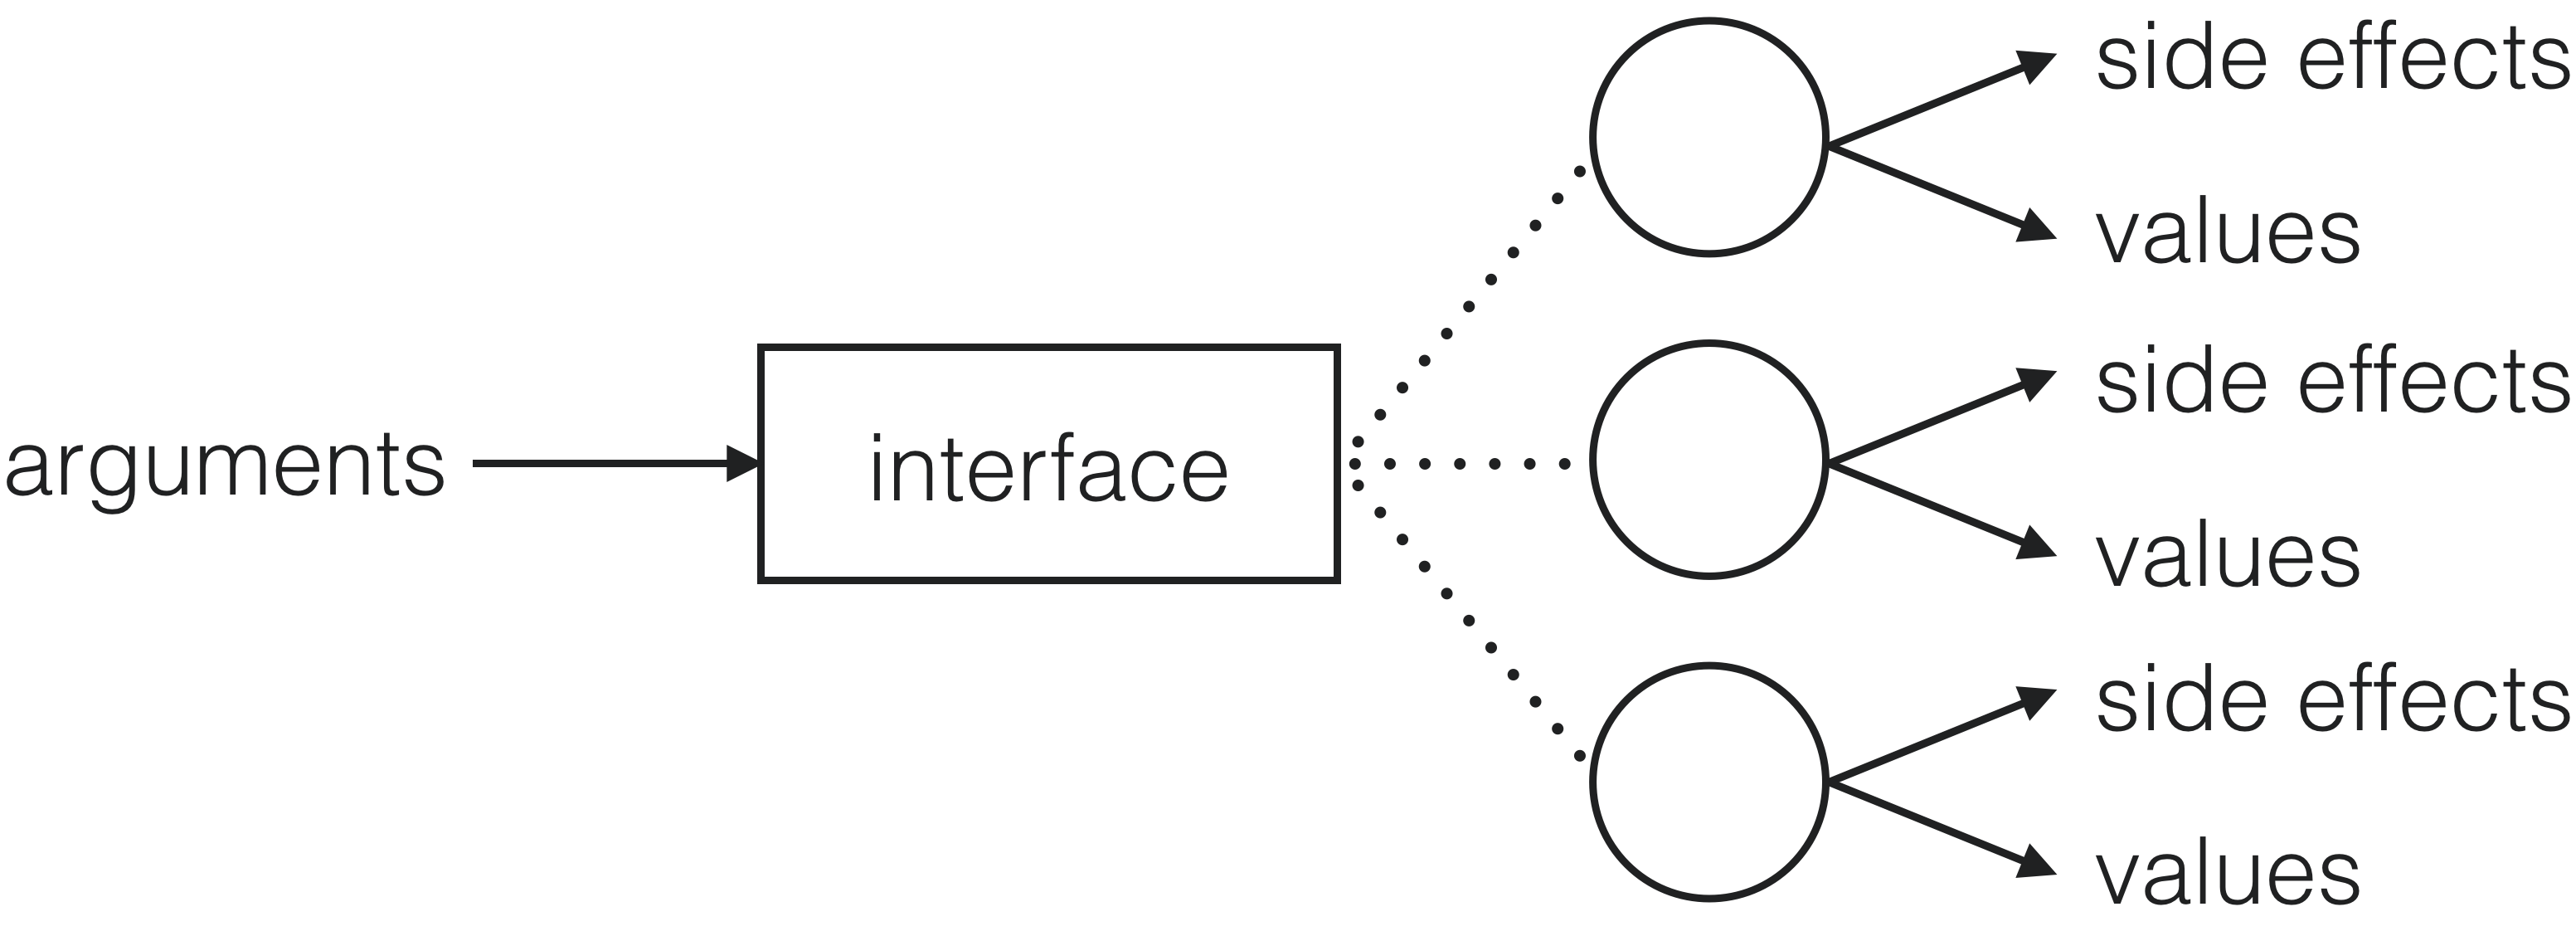
\includegraphics[width=0.53\textwidth]{images/genericfunction.png}
    \caption{The global interface provided by the generic function}
    \label{fig:genericfunction}
\end{figure}

\section{Approach and Implementation}
\label{sec:approach}

As discussed in Section \ref{sec:oo}, Object Orientation is suitable for the description of real world states of affairs. Together with its concepts, CLOS thus lends itself to the creation and maintenance of descriptions of organizational structures.

In our solution, classes represent the roles, while an instance of such a class would be an individual member of the organization. This way, a Lisp REPL can be used for simple queries, while other Lisp-programs (such as human capital management software) could use the objects for further interaction. CLOS furthermore permits the storage of objects in SQL database systems via object-relational mappers\footnote{A list of object-relational mappers for CLOS can be found at \url{http://www.cliki.net/ORM}, missing from the list is Mito (\url{https://github.com/fukamachi/mito}), both accessed: 2016-07-18}, so that non-Lisp programs can also have easy access. Nevertheless, this work focuses on a description of the arrangement of people within an organizational structure and  an interface to query information on individuals and occupations.
\newline

\begin{figure}[]
    \centering
    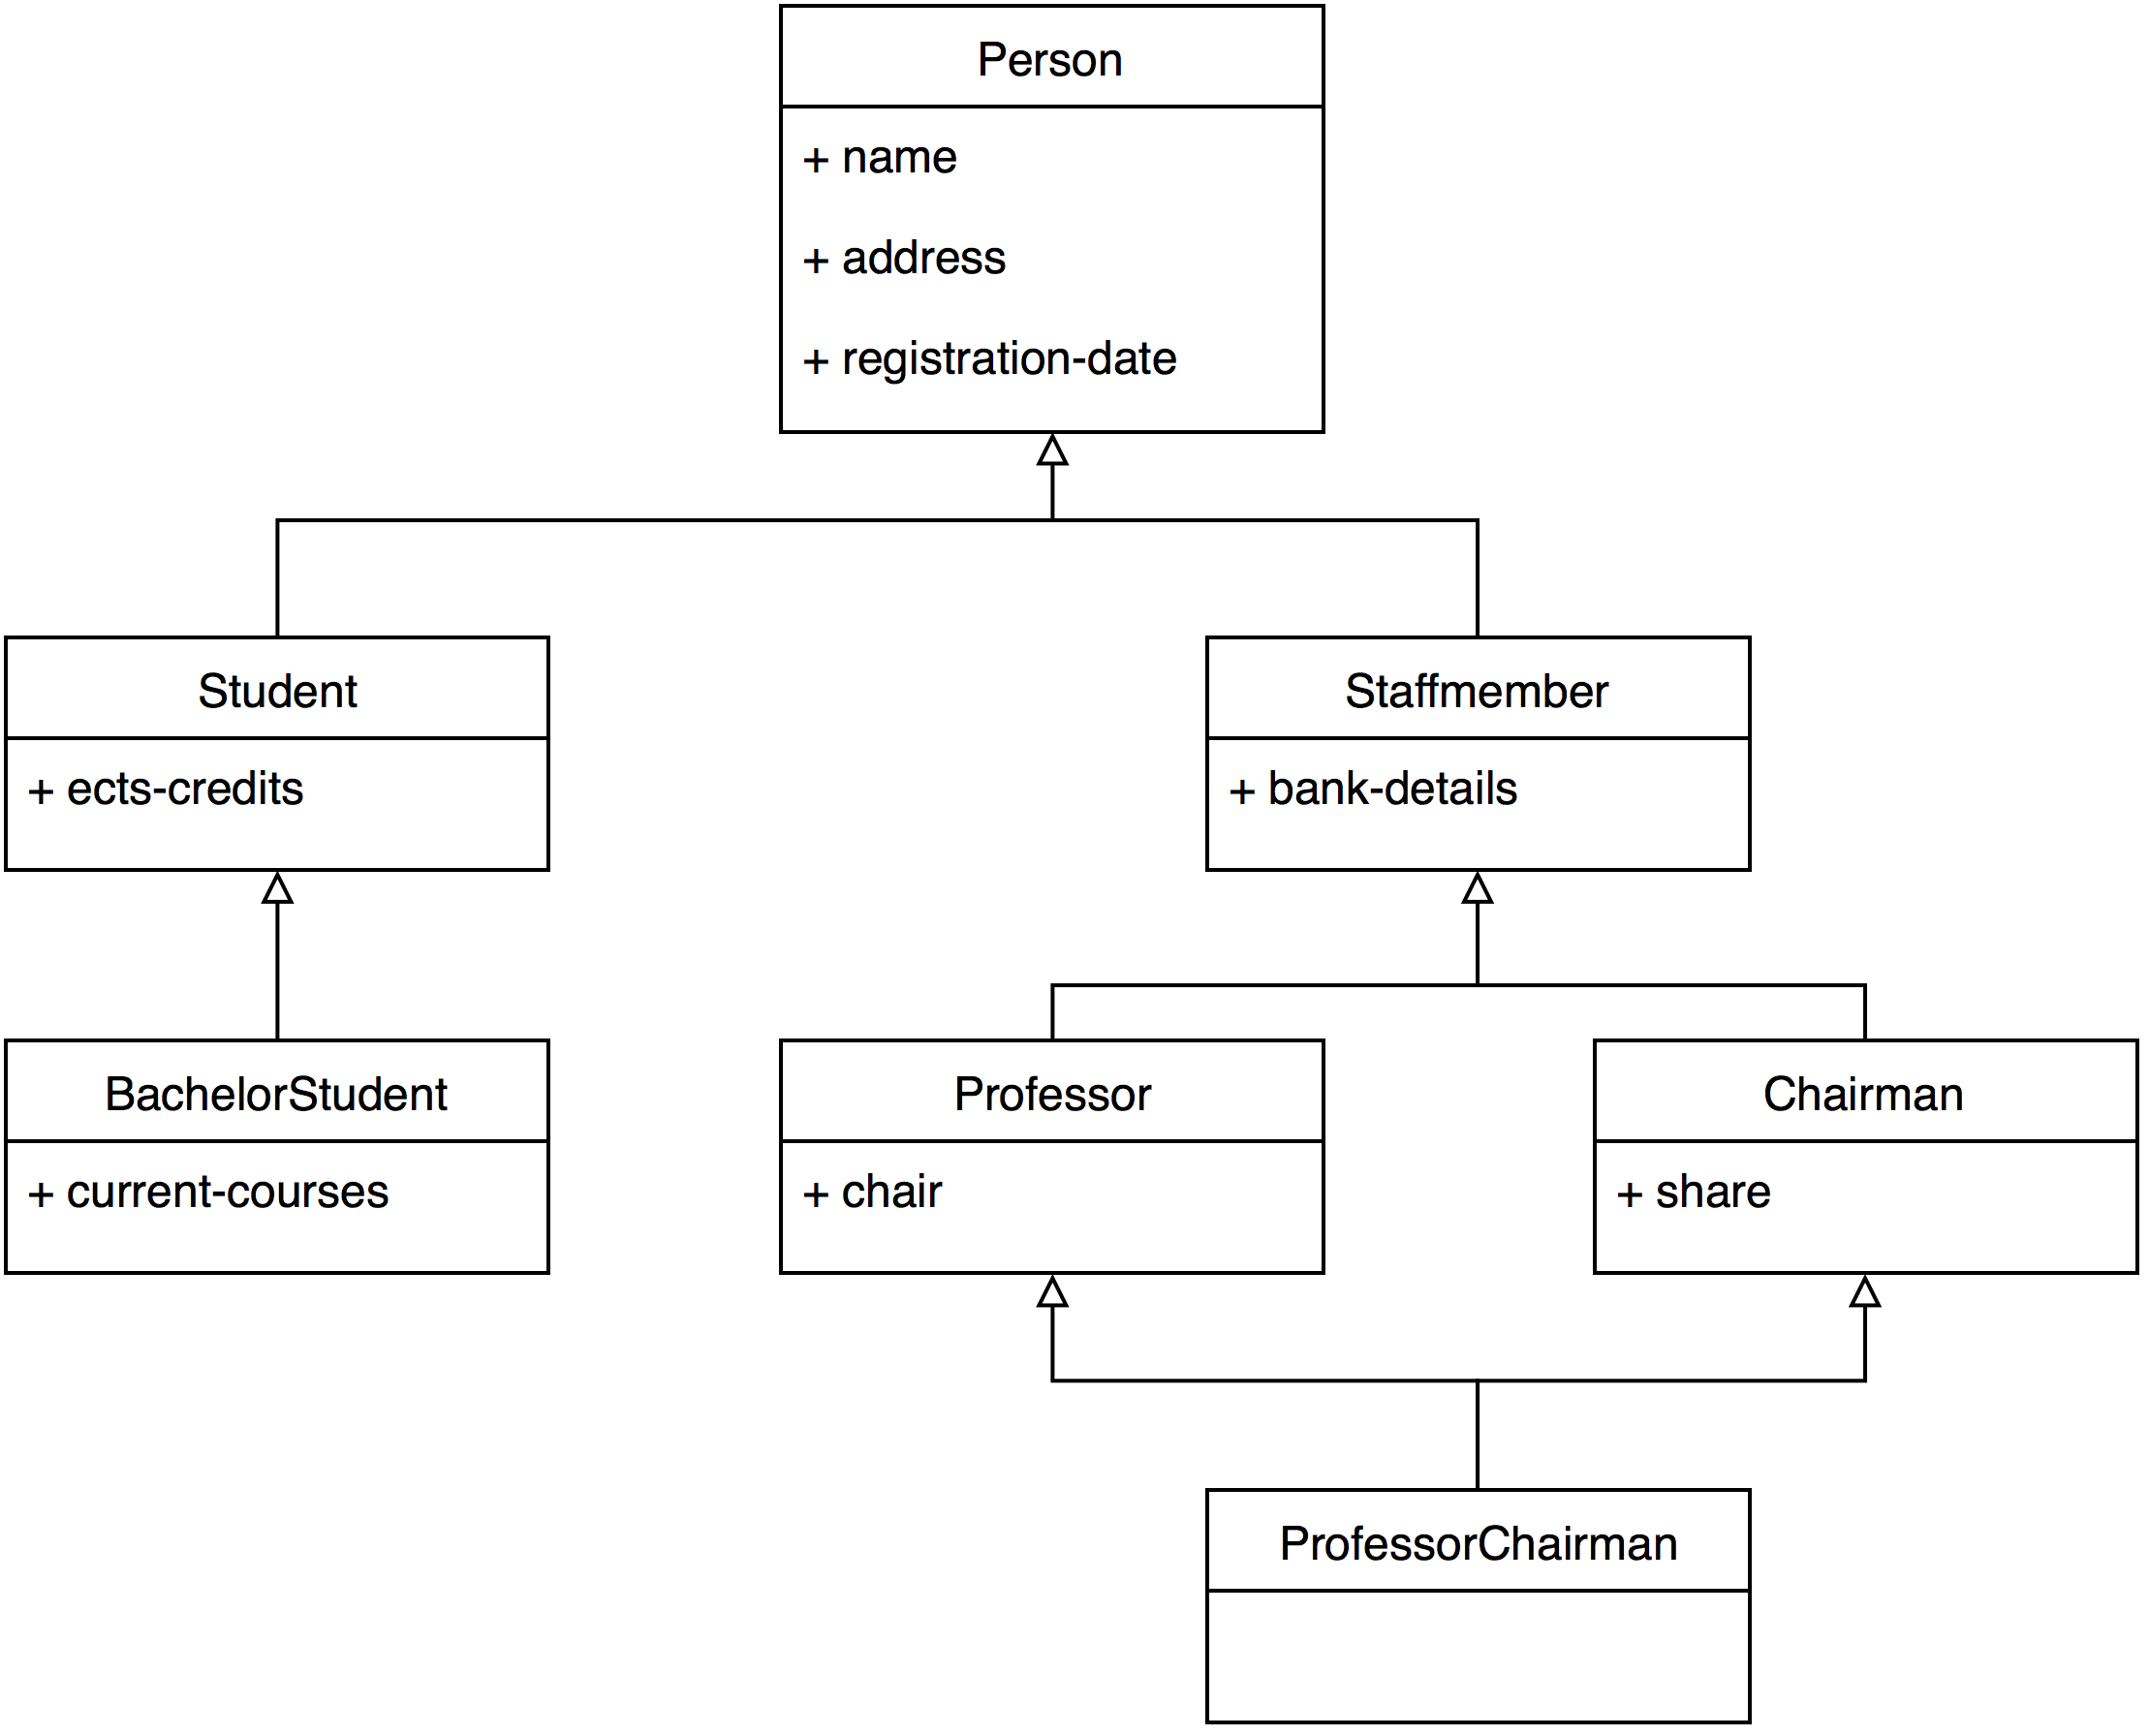
\includegraphics[width=0.83\textwidth]{images/class-diagram.png}
    \caption{Excerpt from a UML class diagram of a description of the occupations within a university}
    \label{fig:class-diagram}
\end{figure}

A common organizational structure is the university, which we will use to exemplify our approach to the general problem presented in Section \ref{sec:problem}. As new students and chairs come and go, new roles and corresponding individuals will have to be accommodated for. The following is an abstract description of a possible arrangement of roles which is visualized in Figure \ref{fig:class-diagram}. 

Since all members have a certain set of common attributes such as name and address, an abstract class \mintinline{lisp}{person} for all members to inherit from will have to exist. Listing \ref{lst:person} shows a possible implementation of such a class. Even though \mintinline{lisp}{person} is an abstract class, it is still possible to instantiate it. However, since such a \mintinline{lisp}{person} object would not provide any meaning to the overall system, our approach omits any helper method in the form of \mintinline{lisp}{make-person} or the like.

\begin{listing}[]%ht]
    \centering
\begin{minted}{lisp}

(defclass person ()
  ((name :accessor name
         :initarg :name)
   (age :accessor age
        :initarg :age)
   (address :accessor address
         :initarg :address)
   (registration-date :accessor registration-date
         :initarg :registration-date)))
\end{minted}
\caption{The basic \mintinline{lisp}{person} class}
\label{lst:person}
\end{listing}

A distinction between students and staff members would make sense, since the staff needs bank details for compensations. In reality however, this line is blurred by multiple inheritance, as a student might also at some point become a research assistant. A \mintinline{lisp}{staffmember} class would, just like \mintinline{lisp}{person}, again be abstract to facilitate the centralization of common attributes and behaviors. Such a distinction will obviously be unnecessary in other organizations, but it helps in making sense of the inherent structures. Listing \ref{lst:student} shows the definition of the \mintinline{lisp}{student} and \mintinline{lisp}{staffmember} classes, which both inherit from student. As \mintinline{lisp}{student} is not an abstract class, it is useful to create an easy-to-use \mintinline{lisp}{make-student} function, since the \mintinline{lisp}{make-instance} function can be felt to be rather tedious to work with.

\begin{listing}[]%ht]
 \centering
\begin{minted}{lisp}

(defclass student (person)
 ((ects-points :accessor ects-points
           :initarg :ects-points)))

(defun make-student (name age address registration-date ects-points)
 (make-instance 'student :name name :age age :address address
    :registration-date registration-date :ects-points ects-points))
    
    
(defclass staffmember (person)
  ((bank-details :accessor bank-details
            :initarg :bank-details)))

\end{minted}
\caption{The definition of the \mintinline{lisp}{student} and \mintinline{lisp}{staffmember} classes}
\label{lst:student}
\end{listing}


As it is possible that a member of an organization can take on multiple roles within the structure, classes will need to be able to have multiple superclasses. An example would be the university's chairman who also happens to be a professor. In our solution, this is possible through CLOS' concept of multiple inheritance. As shown in Listing \ref{lst:chairmanprof}, \mintinline{lisp}{professor-chairman} would simply be a subclass of both \mintinline{lisp}{professor} and \mintinline{lisp}{chairman}\footnote{The instantiation interfaces like \mintinline{lisp}{make-professor} have been omitted to declutter the code. In an actual implementation however they should exist as well.}. Here it is important to make sure that the order in which the superclasses are declared is in such a way that in the case of duplicate methods or attributes, the superclass named first is the one to have priority. If prioritization however is not desired, then the naming will have to be adjusted.

\begin{listing}[]%ht]
 \centering
\begin{minted}{lisp}
(defclass professor (staffmember)
  ((chair :accessor chair
            :initarg :chair)))

(defclass chairman (staffmember)
  ((share :accessor share
            :initarg :share)))

(defclass professor-chairman (professor chairman) () )

\end{minted}
\caption{The definition of the \mintinline{lisp}{professor}, \mintinline{lisp}{chairman}, and \mintinline{lisp}{professor-chairman} classes}
\label{lst:chairmanprof}
\end{listing}

When making queries via a Lisp REPL\footnote{\emph{Read-Evaluate-Print Loop}}, a simple interface should make responses that should share a common format. And since the addition of new occupations should not require any alterations to such an interface, the method combination concept would prove its usefulness. As can be seen in Listing \ref{lst:interface}, the generic function is defined first via \mintinline{lisp}{defgeneric}, and then the individual implementations for each class are defined. With \mintinline{lisp}{:after}, each additional class can concatenate a particular own behavior to the general behavior of its superclass(es).

\begin{listing}[]%ht]
 \centering
\begin{minted}{lisp}
(defgeneric get-info (person)
      (:documentation "Returns data on all attributes."))

(defmethod get-info ((p person))
    (format t "Name: ~d ~% Occupation: ~d ~% Age: ~d ~% 
     Address: ~d ~% Date of Registration: ~d ~% "
     (name p) (class-of p) (age p) (address p) (registration-date p)))

(defmethod get-info :after ((s student))
    (format t "ECTS Points: ~d ~% " (ects-points s)))

(defmethod get-info :after ((s staffmember))
    (format t "Bank Details: ~d ~% " (bank-details s)))

(defmethod get-info :after ((p professor))
    (format t "Chair: ~d ~% " (chair p)))

(defmethod get-info :after ((c chairman))
    (format t "Share: ~d ~% " (share c)))

\end{minted}
\caption{The functions for human readable output WIP}
\label{lst:interface}
\end{listing}

Figure \ref{fig:repl} demonstrates a possible interaction with the framework for describing organizational structures.

\begin{figure}[]
    \centering
    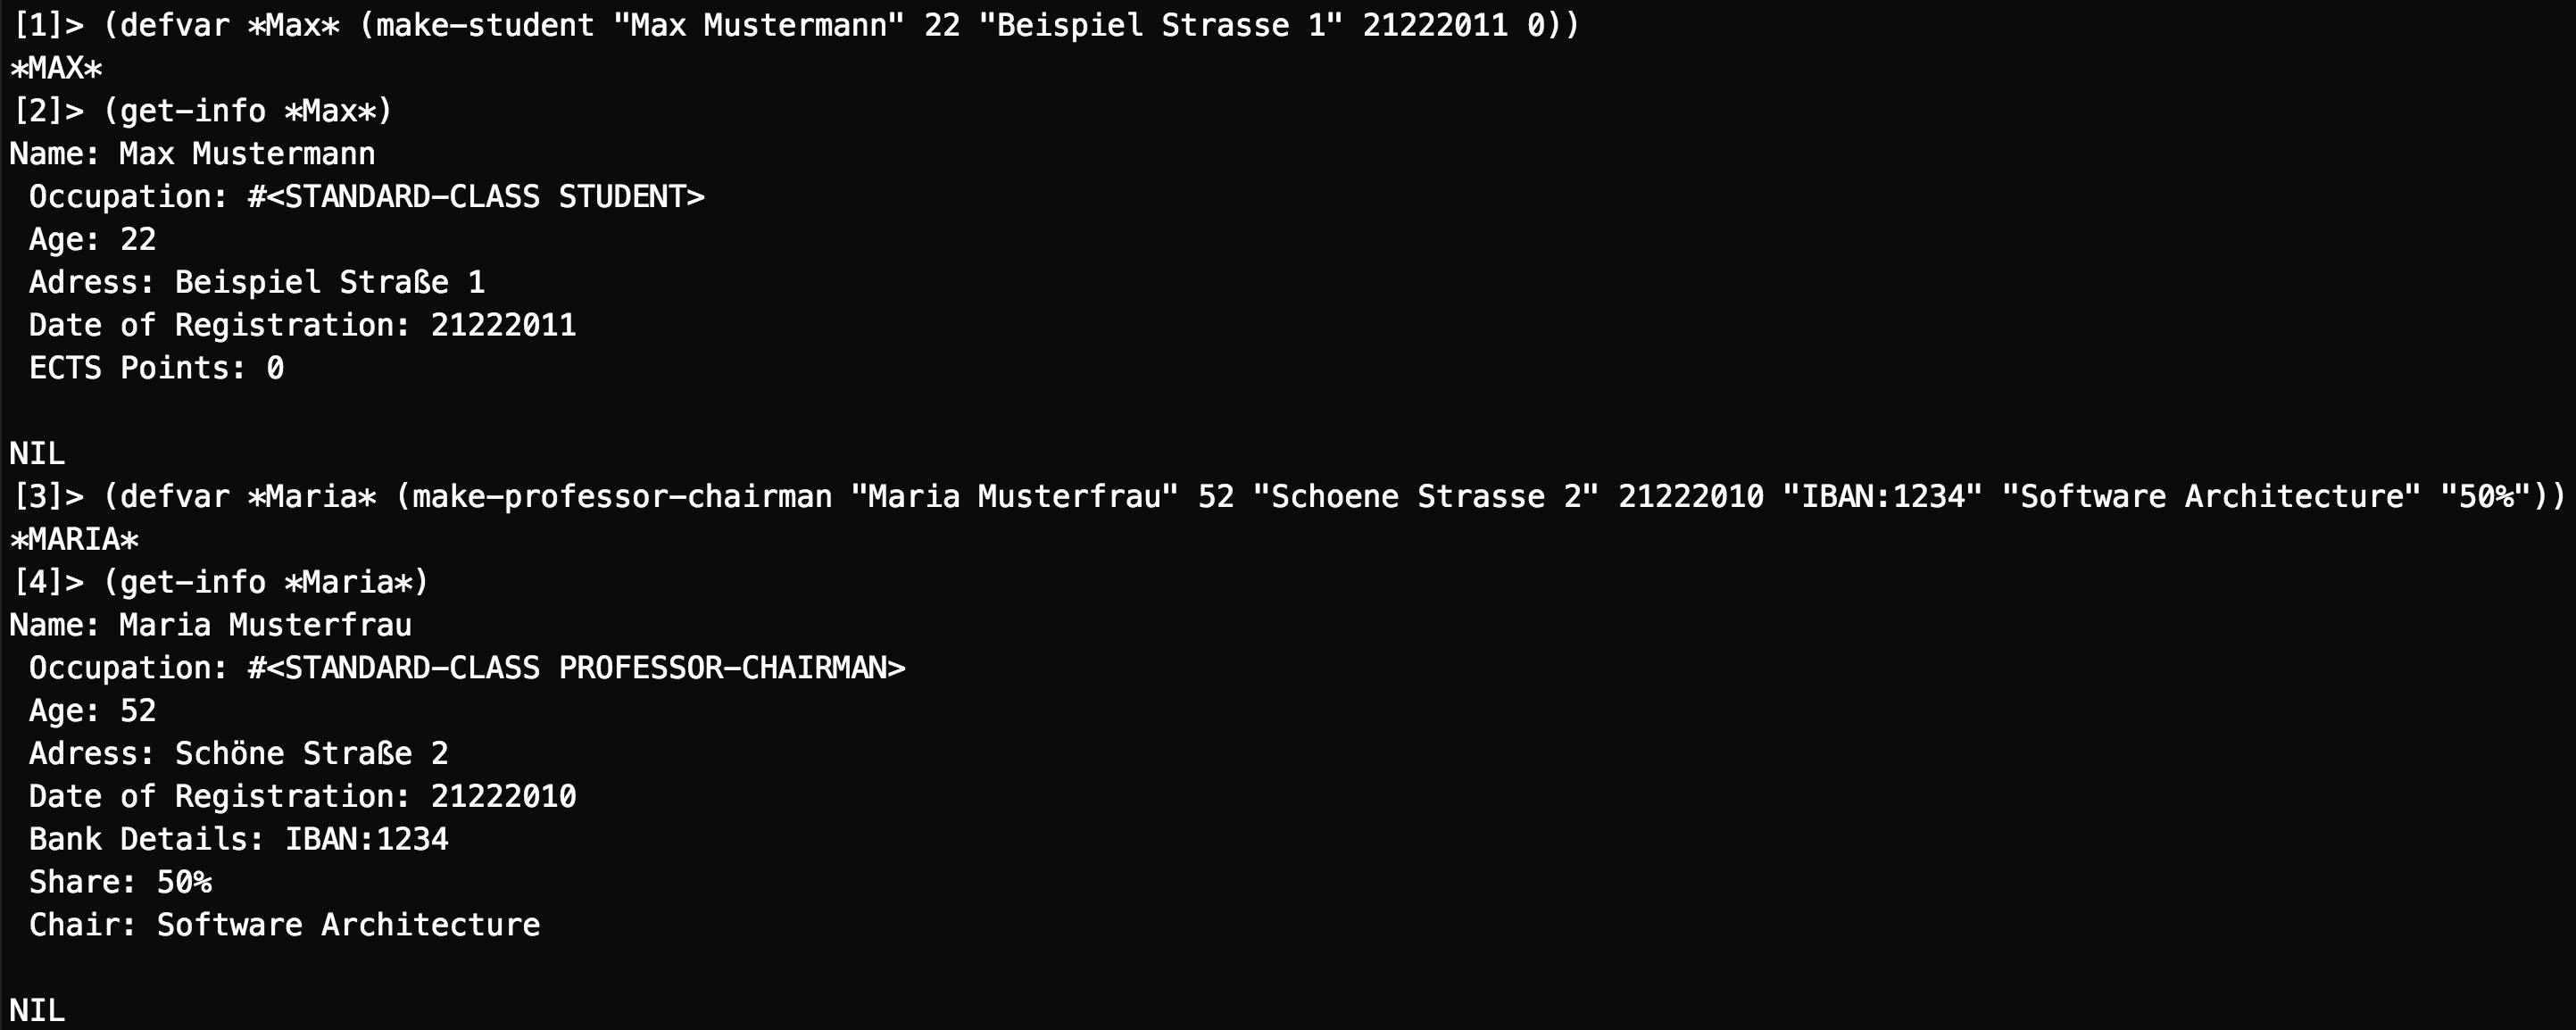
\includegraphics[width=1\textwidth]{images/repl.png}
    \caption{A screenshot of a possible interaction with the framework provided by our solution}
    \label{fig:repl}
\end{figure}


\section{Evaluation}
\label{sec:evaluation}

In Section \ref{sec:problem} we defined as main requirements the three evolution qualities \emph{maintainability}, \emph{extensibility}, and \emph{accessibility}. In this Section we will discuss, whether and to what extent the solution given in Section \ref{sec:approach} can satisfy them.

\subsubsection{Maintainability}
The \mintinline{lisp}{make-CLASSNAME} functions provide an easy to use interface to add new members to the system. The only issue here would be the yet non-existent man-page to exactly know which parameters a class has and in what order they are supposed to be designed. A UI would make this a lot easier. However, the \mintinline{lisp}{age} attribute for example is not useful in such a system, since the value will inevitably change over time. To keep it maintainable, a \mintinline{lisp}{date-of-birth} attribute would be more appropriate. 

\subsubsection{Extensibility} 
As CLOS makes it easy to add new classes and combine them, new types of occupations within an organizational structure can be easily added. The concept of inheritance in object-oriented languages facilitates especially. The method combination furthermore facilitated the creation of human readable output functions, which can be concatenated for any additional attribute of a new class. 

\subsubsection{Accessibility}
Since CLOS is standardized, any Lisp program can make use of the proposed framework. Objects can be reused in other programs and though the help of object-relational mappers, other non-Lisp programs can also access the information within the system.
\newline

Our solution shows that CLOS as example of Object Orientation lends itself very well to the description of real world states-of-affairs. It is a powerful extension of the Lisp programming language and gave a good impression of what was to expect from object-oriented languages to come.

\section{Related Work}
\label{sec:related}

Today, Object Orientation is a very popular programming concept. Therefore, a plethora of different object-oriented languages exist which could solve the presented problem in their own way. In this Section we will discuss the example of Java, a particularly popular object-oriented programming language.

\begin{listing}[]
\begin{minted}{java}

public interface ProfessorInterface {
}

public class Professor implements ProfessorInterface{
}

public interface ChairmanInterface {
}

public class ProfessorChairman implements ProfessorInterface, ChairmanInterface{
}

\end{minted}
\caption{An example of multiple inheritance using Java interfaces}
\label{lst:java}
\end{listing}

Java does not have multiple inheritance integrated as directly as CLOS does, meaning that because of the diamond problem unwanted behavior can arise during compilation\footnote{\url{https://docs.oracle.com/javase/tutorial/java/IandI/multipleinheritance.html}, accessed: 2016-07-28}. The combination of classes would thus need to be solved in a different manner. Instead, Java \emph{Interfaces} are recommended to be used to achieve a similar effect. An interface is a sort of protocol that can be used by classes. Such an interface could be used as an abstract class, and so multiple interfaces could be implemented for a class that is a combination of others. 

However, such a solution can be a lot less intuitive for the programmer trying to extend the system, since adding a new occupation to the system would require to create a new class and a interface. Furthermore, it could be unclear what sort of behavior would have to be defined in the either the class or the interface. The elegant solution of method combination in CLOS would also not be present in Java. 


\section{Conclusion}
\label{sec:conclusion}

In this work we have discussed the object-oriented Lisp system CLOS by applying it to the problem of member registers of organizations, based on the example of a university. 

First, an introduction to the concepts behind CLOS was given, as well as a description of its history, and its three main ideas, namely \emph{multiple inheritance}, \emph{method combination}, and \emph{generic functions}, were presented. Based on the qualities of \emph{maintainability}, \emph{extensibility}, and \emph{accessibility}, the solution was evaluated and the example of Java as alternative tool was discussed.

\newpage
\nocite{*}
\bibliographystyle{splncs}
\bibliography{hopl-paper}

\newpage
    \begin{center}
      {\bf APPENDIX}
    \end{center}
\label{sec:appendix}

\begin{listing}[]%ht]
\begin{minted}{lisp}
(defclass person ()
  ((name :accessor name
         :initarg :name)
   (age :accessor age
        :initarg :age)
   (address :accessor address
         :initarg :address)
   (registration-date :accessor registration-date
         :initarg :registration-date)))

(defclass student (person)
 ((ects-points :accessor ects-points
           :initarg :ects-points)))

(defclass staffmember (person)
  ((bank-details :accessor bank-details
            :initarg :bank-details)))

(defclass professor (staffmember)
  ((chair :accessor chair
            :initarg :chair)))

(defclass chairman (staffmember)
  ((share :accessor share
            :initarg :share)))

(defclass professor-chairman (professor chairman) () )
\end{minted}
\caption{The implementation of the classes}
\label{lst:entire-implementation}
\end{listing}

\begin{listing}[]%ht]
\begin{minted}{lisp}

(defun make-student (name age address registration-date ects-points)
 (make-instance 'student :name name :age age :address address
    :registration-date registration-date :ects-points ects-points))

(defun make-professor (name age address registration-date bank-details chair)
  (make-instance 'professor :name name :age age :address address
    :registration-date registration-date :bank-details bank-details :chair chair))

(defun make-chairman (name age address registration-date bank-details share)
  (make-instance 'chairman :name name :age age :address address
    :registration-date registration-date :bank-details bank-details :share share))

(defun make-professor-chairman (name age address registration-date bank-details chair share)
  (make-instance 'professor-chairman :name name :age age :address address
    :registration-date registration-date :bank-details bank-details :chair chair :share share))
\end{minted}
\caption{The instantiation functions}
\label{lst:insts}
\end{listing}



\begin{listing}[]%ht]
\begin{minted}{lisp}

(defgeneric get-info (person)
      (:documentation "Returns data on all attributes."))

(defmethod get-info ((p person))
    (format t "Name: ~d ~% Occupation: ~d ~% Age: ~d ~% 
     Address: ~d ~% Date of Registration: ~d ~% "
     (name p) (class-of p) (age p) (address p) (registration-date p)))

(defmethod get-info :after ((s student))
    (format t "ECTS Points: ~d ~% " (ects-points s)))

(defmethod get-info :after ((s staffmember))
    (format t "Bank Details: ~d ~% " (bank-details s)))

(defmethod get-info :after ((p professor))
    (format t "Chair: ~d ~% " (chair p)))

(defmethod get-info :after ((c chairman))
    (format t "Share: ~d ~% " (share c)))

\end{minted}
\caption{The implementation of the human readable interface}
\label{lst:implementation}
\end{listing}


\begin{listing}[]%ht]
\begin{minted}{lisp}

(defvar *Max* 
   (make-student "Max Mustermann" 22 "Beispiel Strasse 1" 21222011 0))

(defvar *Maria* 
   (make-professor-chairman "Maria Musterfrau" 52 "Schoene Strasse 2" 
    21222010 "IBAN:1234" "Software Architecture" "50%"))

(get-info *Max*)
(format t "~%--------------~%~%")
(get-info *Maria*)


\end{minted}
\caption{Examples to test the framework}
\label{lst:examples}
\end{listing}

\end{document}